\documentclass[a4paper, 12pt]{article}
\usepackage[utf8]{inputenc}
\usepackage{physics}
\usepackage{hyperref}
\usepackage{amsmath}
\usepackage{float}
\usepackage{graphicx}

\author{Mikael B. Kiste}
\title{FYS3150 project 4 - Ising model}

\newcommand{\expect}[1]{\langle #1 \rangle}

\begin{document}
\maketitle

\abstract{A numerical study on the temperature dependency of ferromagnets in accordance with the Ising model has been conducted by utilizing the Monte Carlo method and the Metropolis algorithm
	
\tableofcontents \newpage

\section{Introduction}
	In its essence, the two dimensional Ising model of a ferromagnet takes into consideration a lattice of dipoles that can either be spin up or spin down. A ferromagnet can reduce its internal energy by aligning spins (consequentially yielding a net magnetization), however, at higher temperatures, the 'randomizing' effects of entropy dominates. A description of the interplay between these to effects is achieved through Helmholtz free energy; and a thermodynamic equilibrium is reached when this free energy is minimized. The experimental results illustrates how the energy at equilibrium\footnote{More specifically the average energy values sampled for a system over a significant period of time} changes as a function of temperature and also the relative relaxation time for different systems.
	The simple 2x2 lattice is first considered as it is relatively simple to solve it analytically. This allows for a comparison between analytical and numerical results.
	Later we solve for lattices of increasing size, which greatly increases complexity and computational requirements.

	\newpage

\section{Theory}
\subsection{The Ising Model}
	In the two dimensional Ising model we consider a lattice of dipoles that are allowed one of two spins, up or down. This restriction means that the model does break down to some degree at low temperatures, but fortunately is more accurate near the Curie temperature.\cite[p.~340]{schroeder} It does not take into account long range interactions but rather each dipole interacts with its neighbors, four in our 2D case. Despite its simplicity the model does manage to predict the phase transition where the ferromagnet becomes a paramagnet at a sufficiently high critical temperature, famously called the Curie temperature, $T_C$. A general analytical solution of the partition function for the two-dimensional Ising model on a square lattice was solved in the 1940s by Lars Onsager\cite[p.~343]{schroeder}. This solution however is way beyond the scope of this project. Instead only the simple 2x2 will be solved analytically and numerical techniques will be utilized for larger systems.\\
	Note that periodic boundary conditions are used for all the simulations. Essentially meaning that dipoles on the border of the lattice treats dipoles on the opposite side as its neighbor instead. This can be pictured as placing the lattice on the surface of a sphere so that there really is no definitive border, but rather the lattice is closed in on itself. 
	The energy and magnetization are two important quantities. Simplistically we can express the energy of a microstate as a sum over all immediate neighbor dipoles
	\begin{equation}\label{eq:energy}
		E_i = -J\sum_{<kl>}^N s_k s_l
	\end{equation}
	Such that neighbors with opposing spin contributes with $J$ to the total energy and aligned spin contributes with $-J$. Here J acts as a coupling constant.\\
	The magnetization is simply a sum over all the spins themselves. Opposing spin cancel out and the average magnetization is given as the surplus of spin in one of the two directions.
	\begin{equation}
		M_i = \sum_k^N s_k
	\end{equation}
	The system acts according to the Boltzman distribution where the partition function is found to be
	\begin{equation}
		Z = \sum_ie^{-E_i\beta}
	\end{equation}
	Which is a sum over the energies for all possible microstates. Since an nxn lattice has a total of $2^{n^2}$ possible microstates, and the  energy for each of those is a sum over $n^2$, brute calculation of the partition function for large systems is impossible. Instead we utilize the Monte Carlo method.
\subsection{Monte Carlo Method}
	In our simulation we create a subset out of the total amount of microstates achievable with a bias towards favored states. This allows us to calculate average energy, magnetization and other thermodynamic quantities for samples that are statistically representable for the real case. Discarding unlikely states that are energetically unfavored and do not contribute significantly allows for an extremely more efficient numerical solution, this technique is also called Monte Carlo summation with importance sampling\cite[p~347]{schroeder}. In this project this is done through the metropolis algorithm which, for each Monte Carlo cycle, runs through the entire lattice and for each spin evaluates if flipping the spin is favorable according to Helmholtz free energy. It does this by comparing the energy lost due to nearest neighbor interactions, in which case it automatically flips the spin, and with a chance of flipping the spin even if it increases the energy. This chance is temperature dependent, with higher temperatures increasing the likelihood of a flip. This is also where we incorporate the Boltzman distribution to our sampling as the probability is given by
	\begin{equation*}
		P(flip s_j) = e^{- \Delta E_j \beta }
	\end{equation*}
	Where $\Delta E_j = 2Js_j\sum_k s_k$.
	This is a seemingly innocent calculation but since it will be performed so many times and  computing the exponential is so demanding that precalculating the values will save us a significant amount of FLOPS (floating point operations).
	\subsubsection{Precalculation of flip probability}
		We know that each dipole considers only its four neighbors. We also know that flipping all five spins has no effect on the change in energy. 
		\begin{equation*}
			\Delta E_j =  2Js_j\sum_k s_k =  -2Js_j\sum_k -s_k
		\end{equation*}
		Also, because of the commutative nature of the additions in the summation we know that the order/position of the neighboring spins is irrelevant. All this boils down to 5 scenarios with different energies.
		
		\begin{center}
		\begin{tabular}{ c c c }
			Scenario & spin relations & $\Delta E_j$ \\\hline\\
			All spins aligned & $s_j = s_k$ & 8J\\
			All spins but one neighbor aligned & $s_j = s_{k1} = s_{k2} = s_{k3} = -s_{k4}$  & 4J\\
			Two neighbors aligned with $s_j$ & $s_j = s_{k1} = s_{k2} = -s_{k3} = -s_{k4}$  & 0\\
			One neighbor aligned with $s_j $& $s_j = s_{k1} = -s_{k2} = -s_{k3} = -s_{k4}$  & -4J\\
			All neighbors have opposing spin to $s_j$ & $s_j = -s_{k1} = -s_{k2} = -s_{k3} = -s_{k4}$  & -8J\\
		\end{tabular}
		\end{center}
		Now we can calculate $P(flip s_j)$ for these five energies at the beginning of the simulation, store them in an array, and simply access this array any time we would like the probability for a flip at a certain energy. This saves us a a large amount of flip FLOPS.

\subsection{The 2x2 lattice}
	Getting a full analytical description for the 2x2 lattice involves finding the partition function, Z, and even all the specific energies and magnetizations related to each of the $2^4=16$ microstates.
	\subsubsection{Analytical solution of energies for the 2x2 lattice}
		In the following will be considered a 2x2 lattice with spins labeled A,B,C and D that is either spin up or spin down.
		\begin{center}
		\begin{tabular}{ | c | c | }
		\hline
		A & B \\ \hline
		C & D \\
		\hline
		\end{tabular}
		\end{center}
		Let spin up and spin down be represented by the numbers 1 and -1 respectively. This makes sense when summing over nearest neighbour spin interactions when calculating the energy since opposite spins sum out to zero and equal spins contribute an equal amount of energy (say J) no matter the order.
		Due to symmetries, most energies cancel out and sum out to zero. Let's look at the ones that don't do this:
		\begin{align*}
			E = -J\sum_{kl}^Ns_k s_l \neq 0\\
			-J(A(B+C)+B(A+D)+C(A+D)+D(B+C)) \neq 0\\
			A(B+C)+D(B+C)+B(A+D)+C(A+D) \neq 0 \\
			(A+D)(B+C)+(B+C)(A+D) \neq 0 \\
			2(A+D)(B+C) \neq 0 \\
			A+D \neq 0 \qquad B+C \neq 0 \\
			\implies A=D \quad \mathrm{and} \quad B=C
		\end{align*}
		Here it is assumed that $J\neq 0$ in the division. We use the fact that no factor can be zero when the product is nonzero and, for the last step, we use that the variables can only assume the values 1 or -1.
		So the only microstates with non-zero energies are
		\begin{center}
		\begin{tabular}{  l  c  c  }
			Spin configuration & & Energy \\
			$[1,1,1,1]$	&
			\begin{tabular}{  c  c  }
				$\uparrow$ & $\uparrow$\\
				$\uparrow$ & $\uparrow$
			\end{tabular}
			&	-8J \\ \hline\\
			$[1,-1,-1,1]$	&
			\begin{tabular}{  c  c  }
				$\uparrow$ & $\downarrow$\\
				$\downarrow$ & $\uparrow$
			\end{tabular}
			&	-8J\\ \hline \\
			$[-1,1,1,-1]$	&
			\begin{tabular}{  c  c  }
				$\downarrow$ & $\uparrow$\\
				$\uparrow$ & $\downarrow$
			\end{tabular}
			& 8J\\ \hline \\
			$[-1,-1,-1,-1]$	&
			\begin{tabular}{  c  c  }
				$\downarrow$ & $\downarrow$\\
				$\downarrow$ & $\downarrow$
			\end{tabular}
			& 8J
		\end{tabular}
		\end{center}
		Where the energies are calculated by using formula \ref{eq:energy}  using periodic boundary conditions.
		The remaining 12 microstates has zero energy.
	\subsubsection{Partition function, magnetization and expectation values}
		Finding expectation values is made a lot easier if you have the partition function. Fortunately it is trivial to find it in this specific case as we already have all the energies for the relatively few number of microstates. The partition function is defined as
		\begin{equation}
			Z = \sum_ie^{-\beta E_i}
		\end{equation}
		Which is a sum over all microstates with their corresponding energies and $\beta$ is a variable that is inversely related to temperature. In our case the partition function is
		\begin{align*}
			Z = 2e^{8J\beta}+2e^{-8J\beta}+12
		\end{align*}
		Now that we have the partition function we can calculate common expectation values, starting with the energy
		\begin{align*}
			\langle E \rangle & = - \pdv{\ln{Z}}{\beta}\\
			& = - \frac{1}{Z} \pdv{Z}{\beta} \\
			%&= - \frac{16Je^{8J\beta}-16Je^{-8J\beta}}{2e^{8J\beta} + 2e^{-8J\beta} + 12}\\
			&= - \frac{8\qty(Je^{8J\beta}-Je^{-8J\beta})}{e^{8J\beta} + e^{-8J\beta} + 6}
		\end{align*}
		and in a similar fashion energy squared
		\begin{align*}
			\expect{E^2} = \tfrac{1}{Z} \sum_i {E_i}^2 e^{-E_i\beta}\\
			= \frac{1}{z} \qty(128J^2\qty(e^{E_i\beta} + e^{-E_i\beta}))\\
			= \frac{64J^2\qty(e^{E_i\beta} + e^{-E_i\beta})}{e^{E_i\beta} + e^{-E_i\beta} + 6}
		\end{align*}
		There is a certain symmetry in the system as it has no way of differentiating between spin up or spin down. From this it follows that the expectation value for magnetization, $\langle M \rangle$, must be zero. As is common in such cases we calculate the square and absolute value instead. The magnetization for a microstate $M_i$ is calculated simply by taking a sum over all the spins in this state. 
		$$ \abs{M_i} = A_i + B_i + C_i + D_i $$
		Since two spin up and two spin down yields a net zero magnetization these states do not contribute to the expectation value directly. We are left with the states where all spins are aligned and states where there is a single spin pointing in the opposite direction to the others. Observing that there are four states where a single spin is down and the same for spin up we realize that the multiplicity for states with a single spin misaligned must be 8. We already know all energies for the various states and conveniently enough it appears that for states with equal absolute/squared magnetization they also have equal energies.

		\begin{center}
		\begin{tabular}{c c c c c}
			microstate	&	multiplicity	&	$|M|$	&	$M^2$ 	&	$E_i$\\
			\hline \\
			all aligned	&	2	&	4	&	16	&	-8J\\
			single spin misaligned & 8	&	2	&	4	&	0
		\end{tabular}
		\end{center}

		\begin{align*}
			\langle \abs{M} \rangle & = \tfrac{1}{Z} \sum_{i}\abs{M_i}e^{-\beta E_i} = \frac{2(4e^{8J\beta}) + 8(2e^{0})}{Z} = 
			\frac{4e^{8J\beta}+16}{e^{8J\beta}+e^{-8J\beta}+6}\\
			\langle M^2 \rangle & = \tfrac{1}{Z} \sum_{i}M_i^2e^{-\beta E_i} = \frac{2(16e^{8J\beta}) + 8(4e^{0})}{Z} = 
			\frac{16\qty(e^{8J\beta}+1)}{e^{8J\beta}+e^{-8J\beta}+6}\\
		\end{align*}
		The magnetic susceptibility comes out quite nicely from the following relation
		\begin{equation*}
			\chi = \beta \qty( \expect{M^2} - \expect{M}^2 ) = \beta \frac{16\qty(e^{8J\beta}+1)}{e^{8J\beta}+e^{-8J\beta}+6}
		\end{equation*}
		For clarity when calculating the specific heat capacity let $X = e^{8J\beta}$ and $Y = e^{-8J\beta}$, so that $XY=1$.
		We have 
		\begin{align*}
			\expect{C_v}  = -\frac{1}{kT^2}\qty( \expect{E^2}-\expect{E}^2 )\\
			kT^2\expect{C_v}  = \frac{64J^2(X+Y)}{X+Y+6} - \qty(\frac{8J(X-Y)}{X+Y+6})^2 \\
			 = \frac{(X+Y+6)(64J^2(X+Y)) - (8J(X-Y))^2}{(X+Y+6)^2}\\
			 = \frac{64J^2}{(X+Y+6)^2} (X+Y+6)(X+Y)-(X-Y)^2\\
			 = \frac{64J^2}{(X+Y+6)^2} \qty( X^2+XY+XY+Y^2+6X+6Y-X^2+2XY-Y^2 )\\
			 = \frac{64J^2}{(X+Y+6)^2} \qty( 6X + 6Y + 4 )\\
			\expect{C_v} = \frac{64J^2}{kT^2} \frac{6X + 6Y + 4}{(X+Y+6)^2}
		\end{align*}

	
\newpage
\section{Results}
\subsection{Comparison with analytical results}
	From the formulas of the expectation values solved for the 2x2 lattice we can compare these values, using $T=J=\beta=1$ (in units kT/J), with our numerical averages.
	\begin{center}
	\begin{tabular} {l | c | c }
		MC cycles & 	$\expect{E}$ pr spin & $\expect{|M|}$ pr spin \\ \hline \\
		N/A - Analytical & -1.9959820 & 0.99866073 \\
		$10^5$ & -1.9932000 & 0.99800000\\
		$10^5$ & -1.9960400 & 0.99867000\\
		$10^6$ & -1.9959000 & 0.99859900\\
		$10^7$ & -1.9959180 & 0.99864450\\
		$10^8$ & -1.9959816 & 0.99866149
		%\\$10^9$ & -1.9959776 & 0.99865967\\
	\end{tabular}
	\end{center}
	We can see that the number of montecarlo cycles generally improves the model, making the average of the results come closer and closer to the expectation value. In order to get meaningful data from a system in relative equilibrium only the last half of the montecarly cycles are actually sampled from.

	Below is shown how the energies of four different systems evolve with time. In the first plot is a system at low temperatures and with a completely ordered initial lattice. Then a system with increased temperature and finally two systems in the same plots with the same two temperatures as before but with a randomized initial lattice.
	\begin{figure}[H]
	\begin{center}
		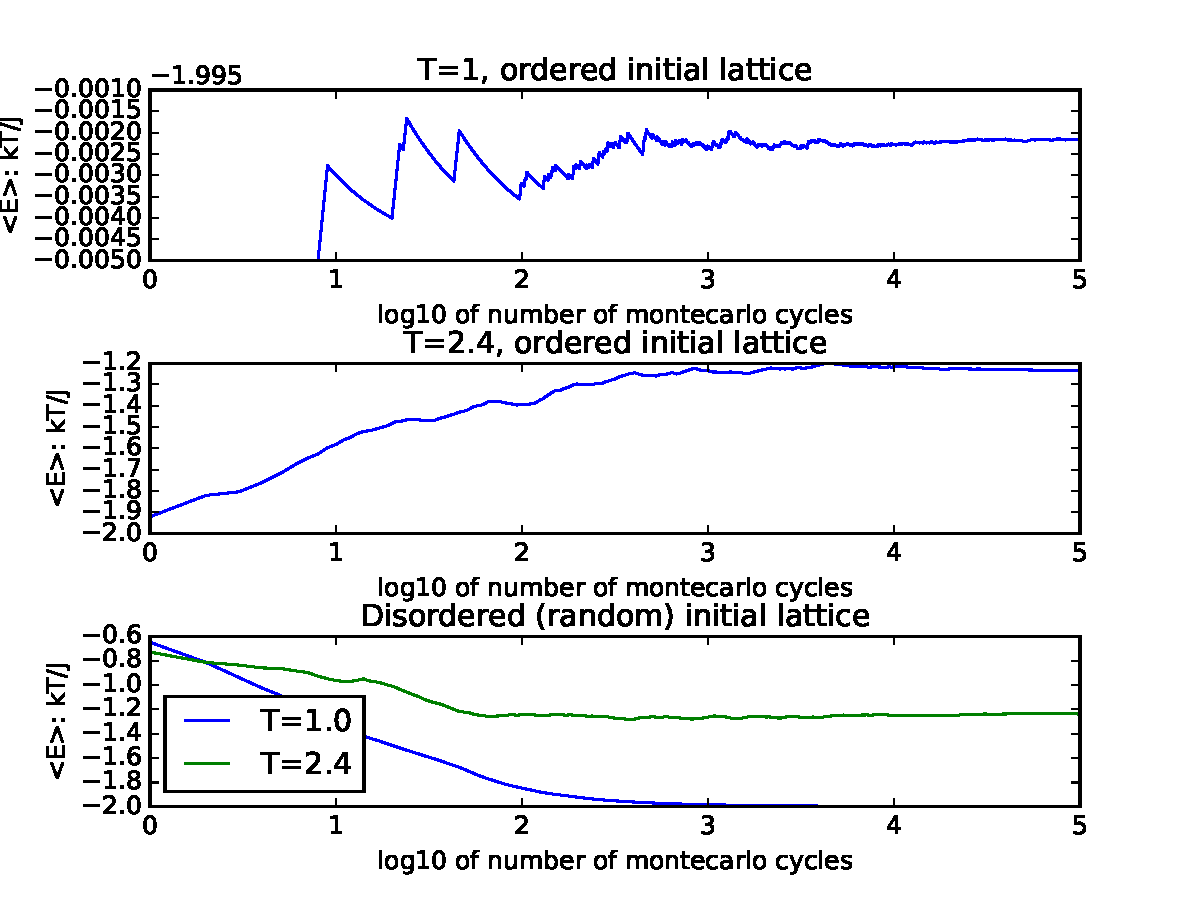
\includegraphics[width=0.9\textwidth]{4c.pdf}
		\caption{Log plots showing expectation value as a function of Monte Carlo cycles for $10^5$ cycles. Both for two different temperatures and differing initial lattice (ordered or random)}
	\end{center}
	\end{figure}
	It is important to note that the x-axis is logarithmic. This way we can clearly see how the energy fluctuates wildly in the beginning before the system has gotten any time to calm down. Another important note is that the y-axis in the first plot shows deviation from -1.995 and therefore only really shows small changes from -2.000 until -1.995. Such small deviations is to be expected when this system practically starts out in a 'preferred' state.

	\newpage
\subsection{Microstates during the relaxation time}
	Looking at the microstates during the relaxation time a bit more closely we can how the system changes over time.
	\begin{figure}[H]
	\begin{center}
		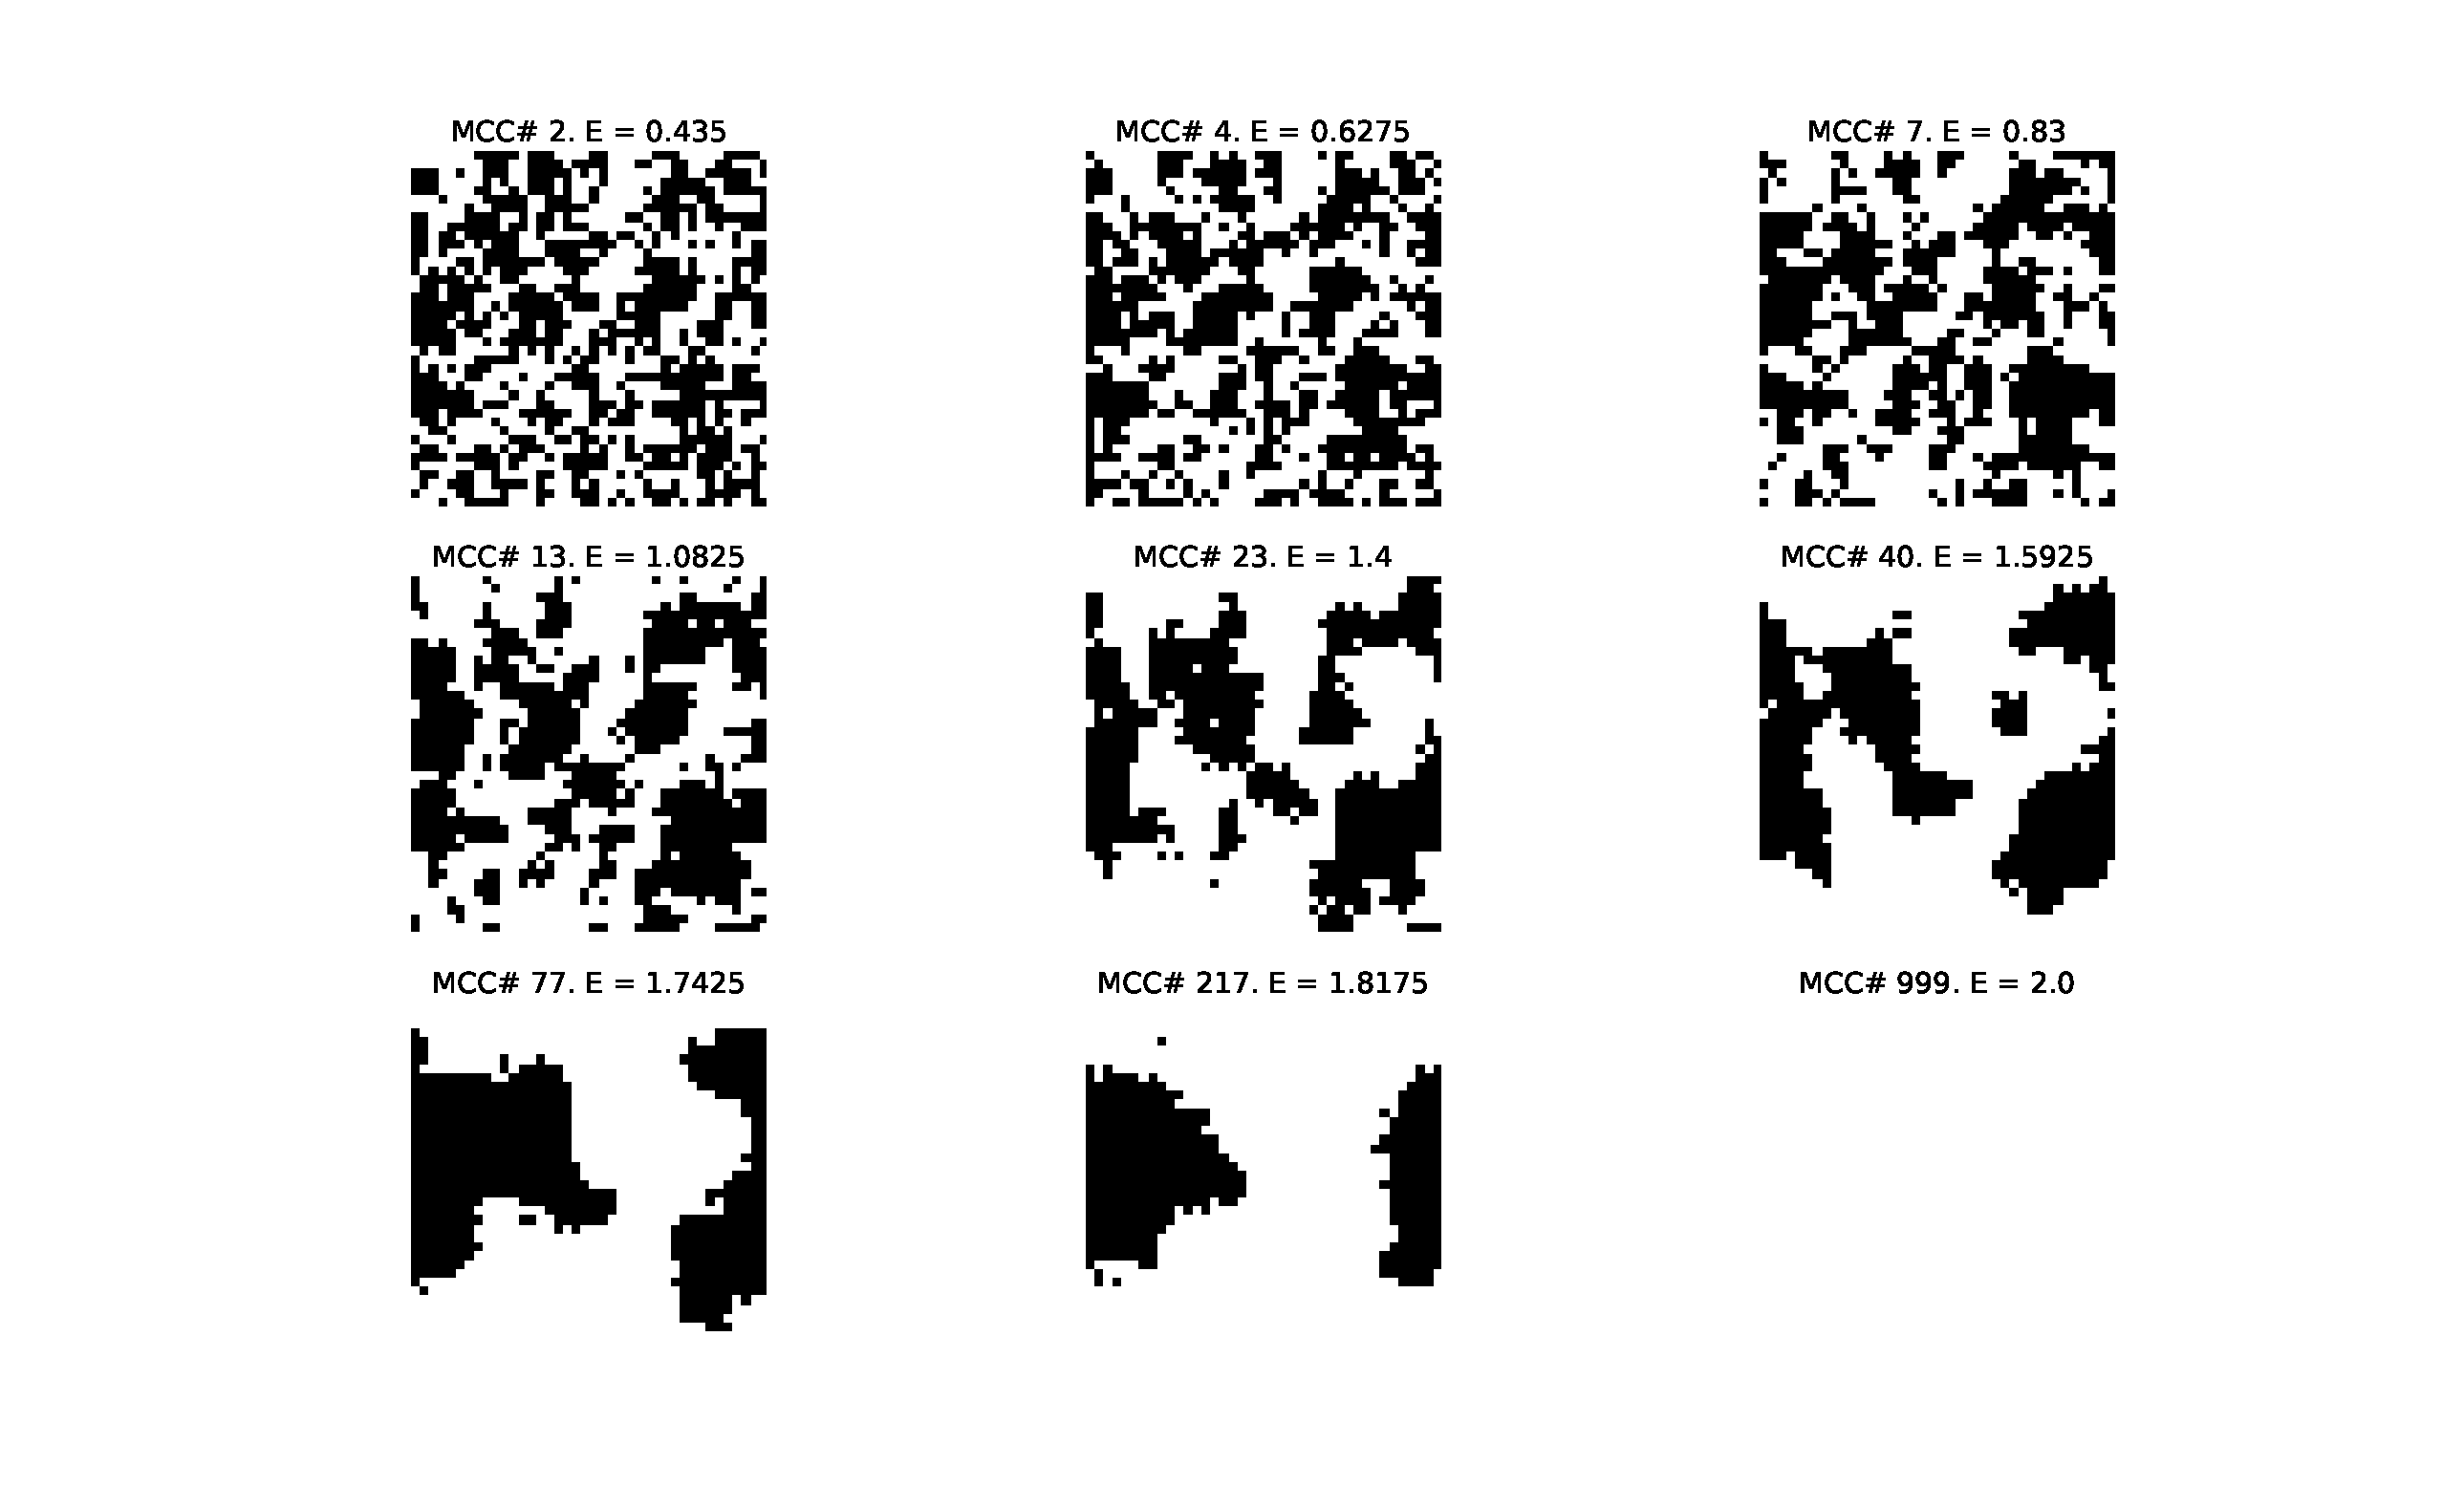
\includegraphics[width=0.8\textwidth]{t1_1000mcc_graphical.pdf}
		\caption{Here we see the system for T=1.0 change as it goes from completely disordered spins until they are completely aligned}
	\end{center}
	\end{figure}
	
	\begin{figure}[H]
	\begin{center}
		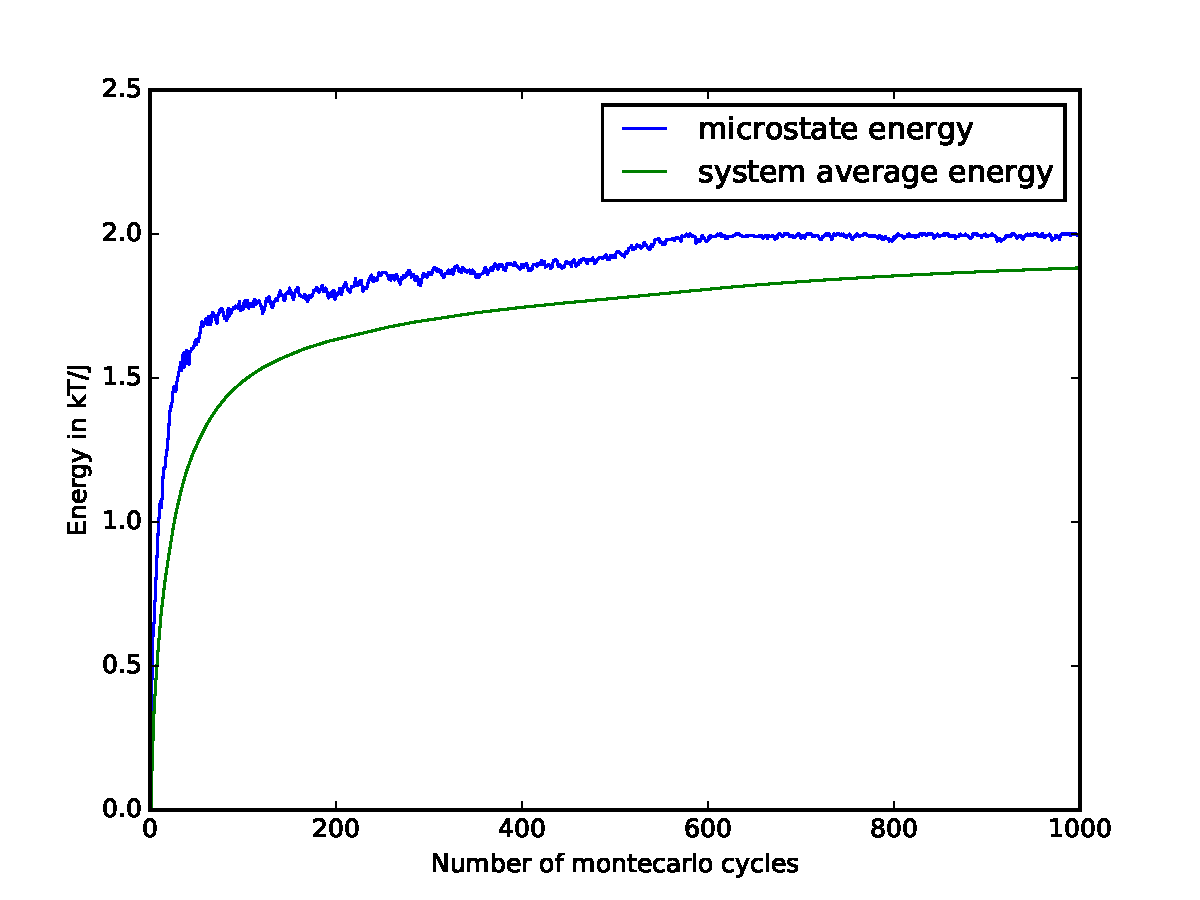
\includegraphics[width=0.5\textwidth]{t1_1000mcc_energies.pdf}
		\caption{In this plot is a plot of the energies for the same system. The y axis shows energy in units kt/J pr dipole ($n^2$). The blue line represents each microstate and the green shows the mean energy for the system up until that point}
	\end{center}
	\end{figure}

	\newpage
	As a comparison we have a completely different case when the temperature is turned up to $T=1.7$.
	\begin{figure}[H]
	\begin{center}
		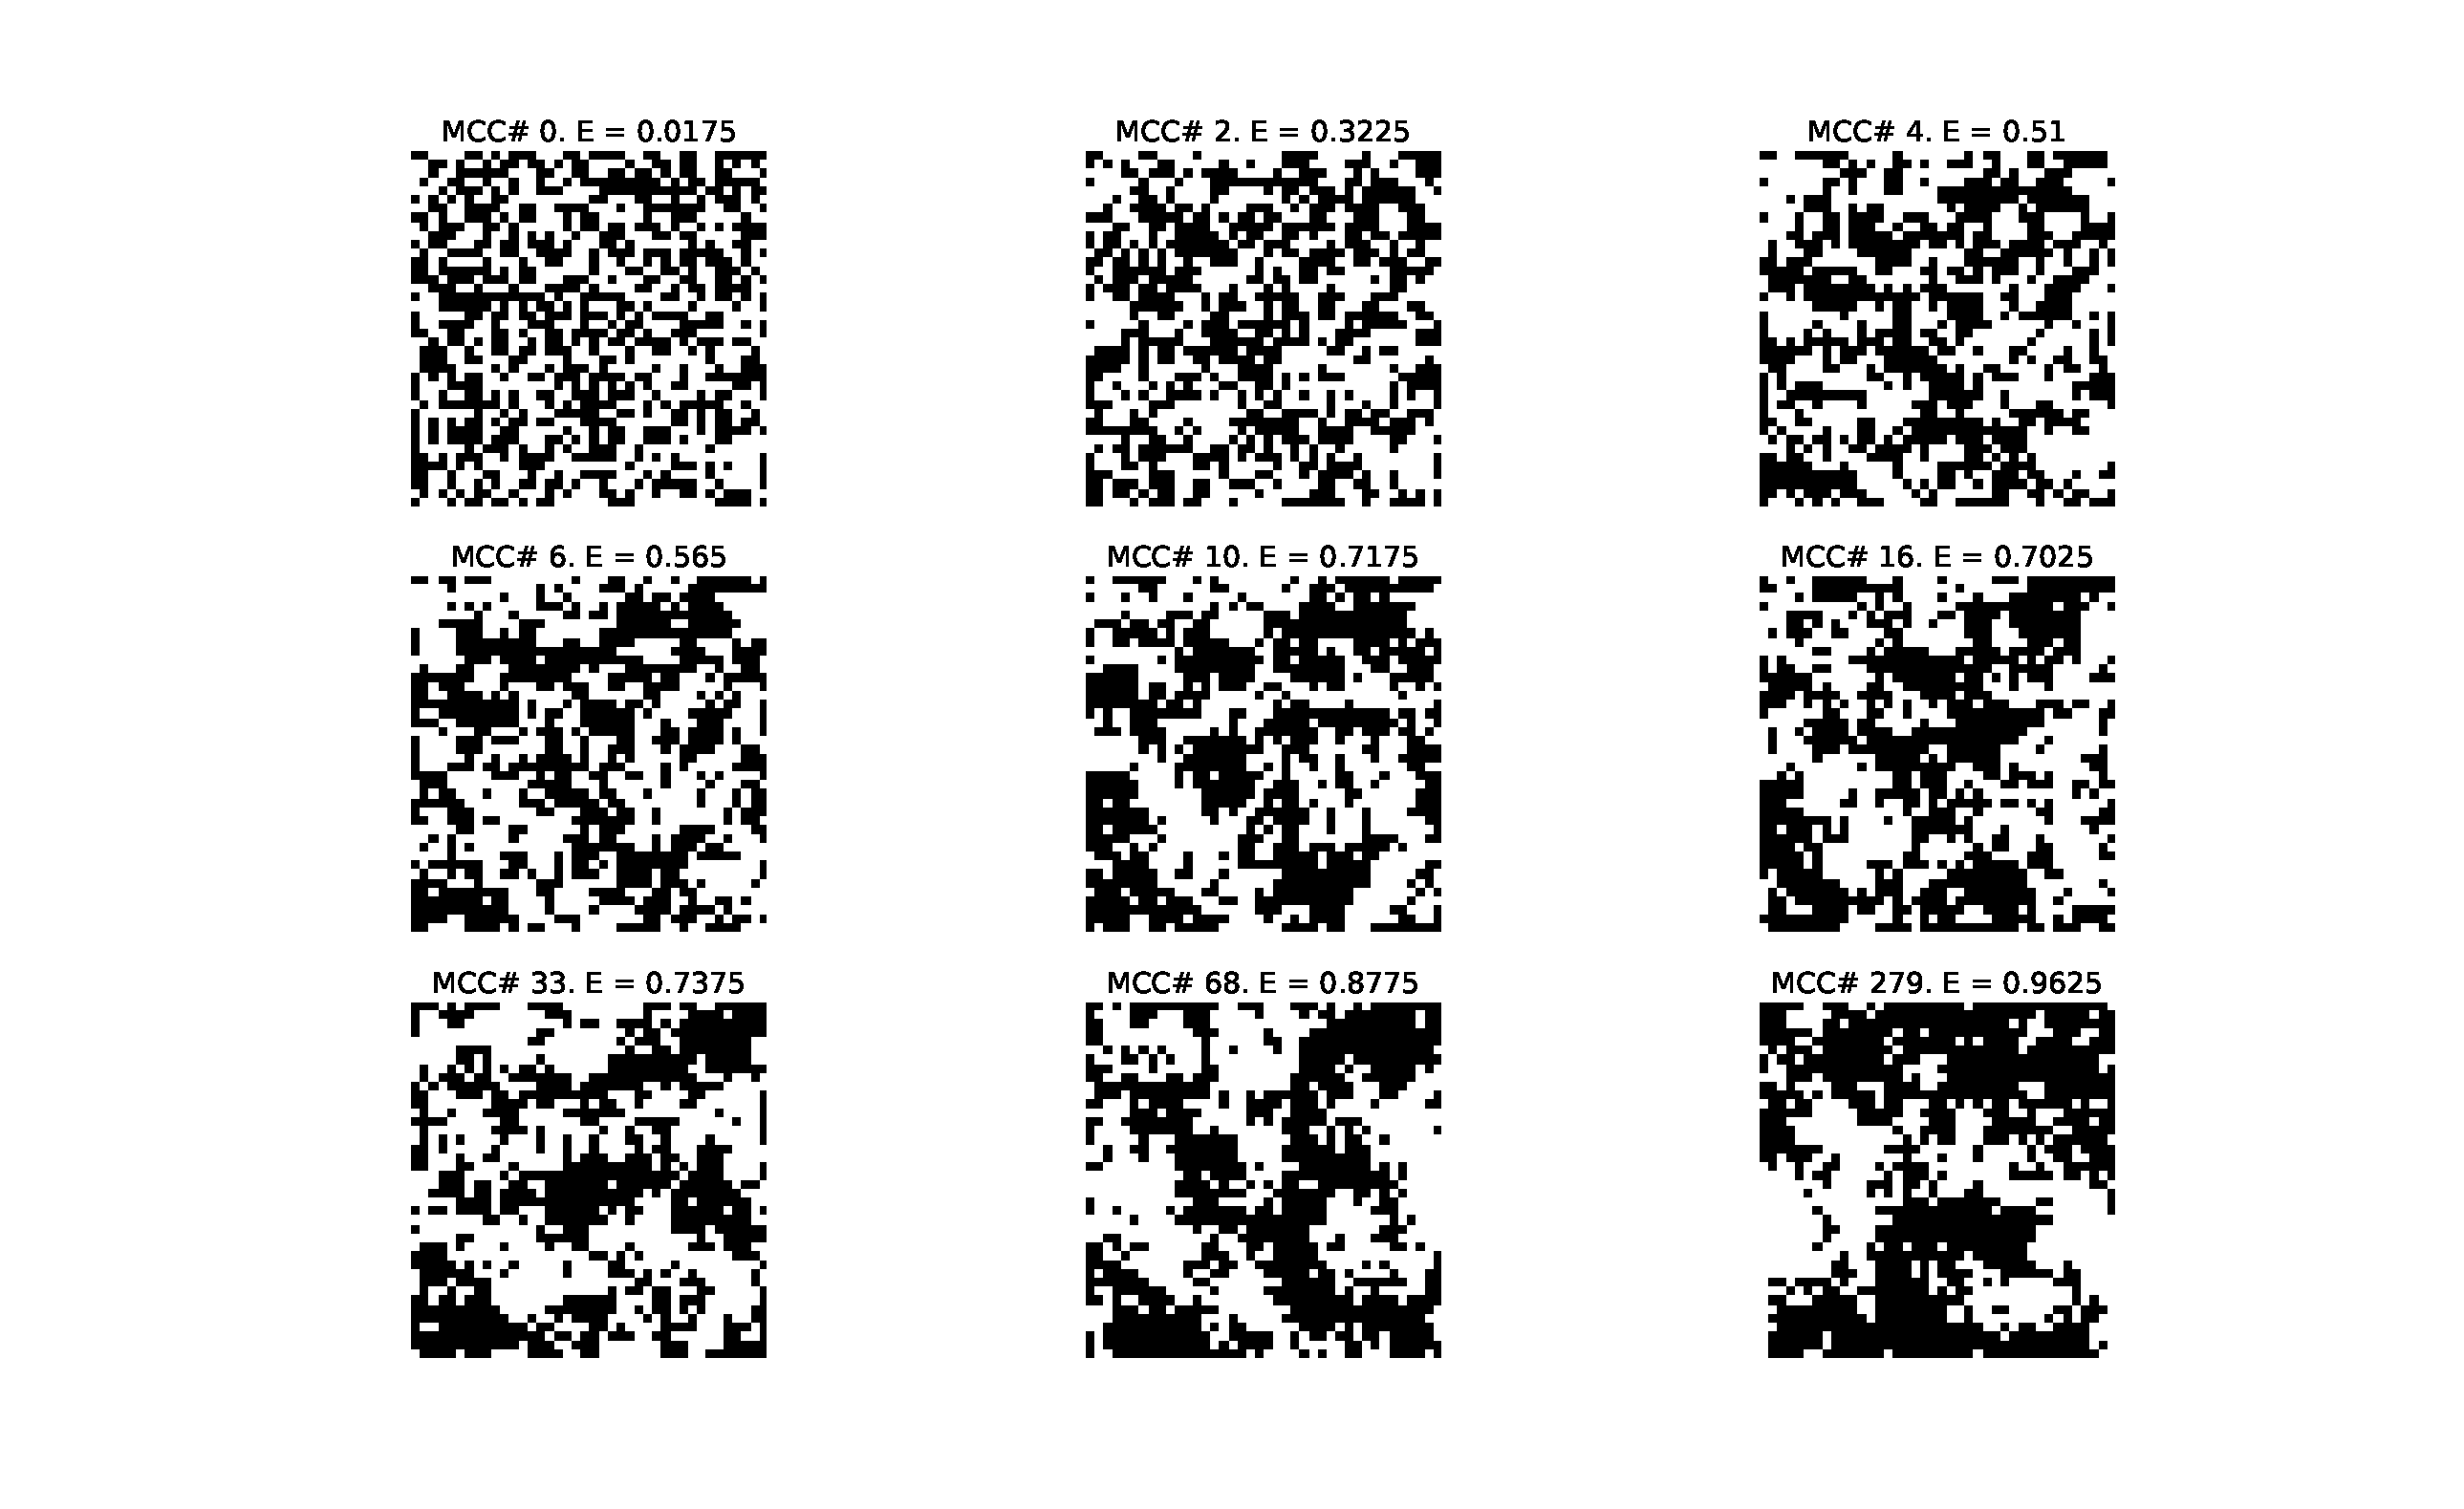
\includegraphics[width=0.8\textwidth]{t17_1000mcc_graphical.pdf}
		\caption{Here we see the system for T=1.7 change as it goes from completely disordered spins to a more ordered state. However it settles at a much more disordered point than for the lower temperature}
	\end{center}
	\end{figure}
	\begin{figure}[H]
	\begin{center}
		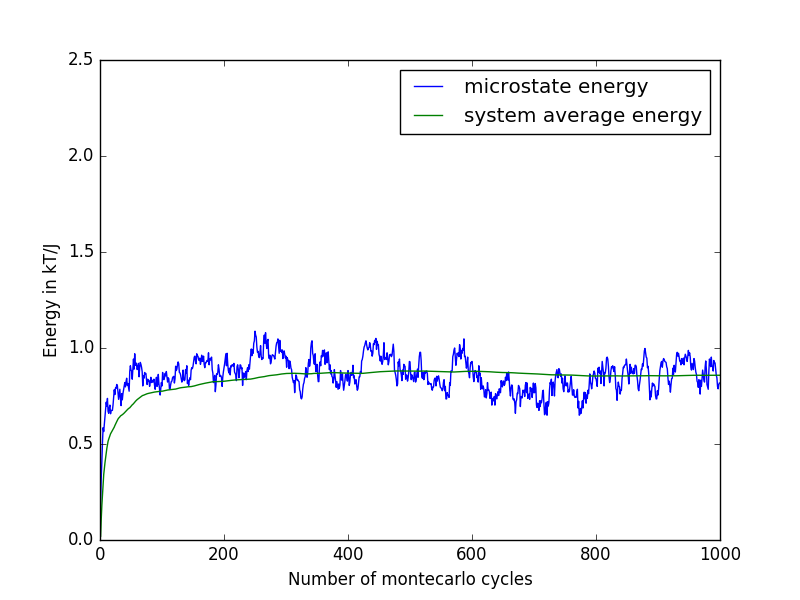
\includegraphics[width=0.5\textwidth]{t17_1000mcc_energies.png}
		\caption{In this plot is a plot of the energies for the same system. The y axis shows energy in units kt/J pr dipole ($n^2$). The blue line represents each microstate and the green shows the mean energy for the system up until that point}
	\end{center}
	\end{figure}

	\newpage
	\subsection{Achievable states after equilibrium is reached}
	We can also look at the system as after it has reached equilibrium. If we plot a histogram of the number of states achieving a certain energy we get a measure of how common these energies are.
	\begin{figure}[H]
	\begin{center}
		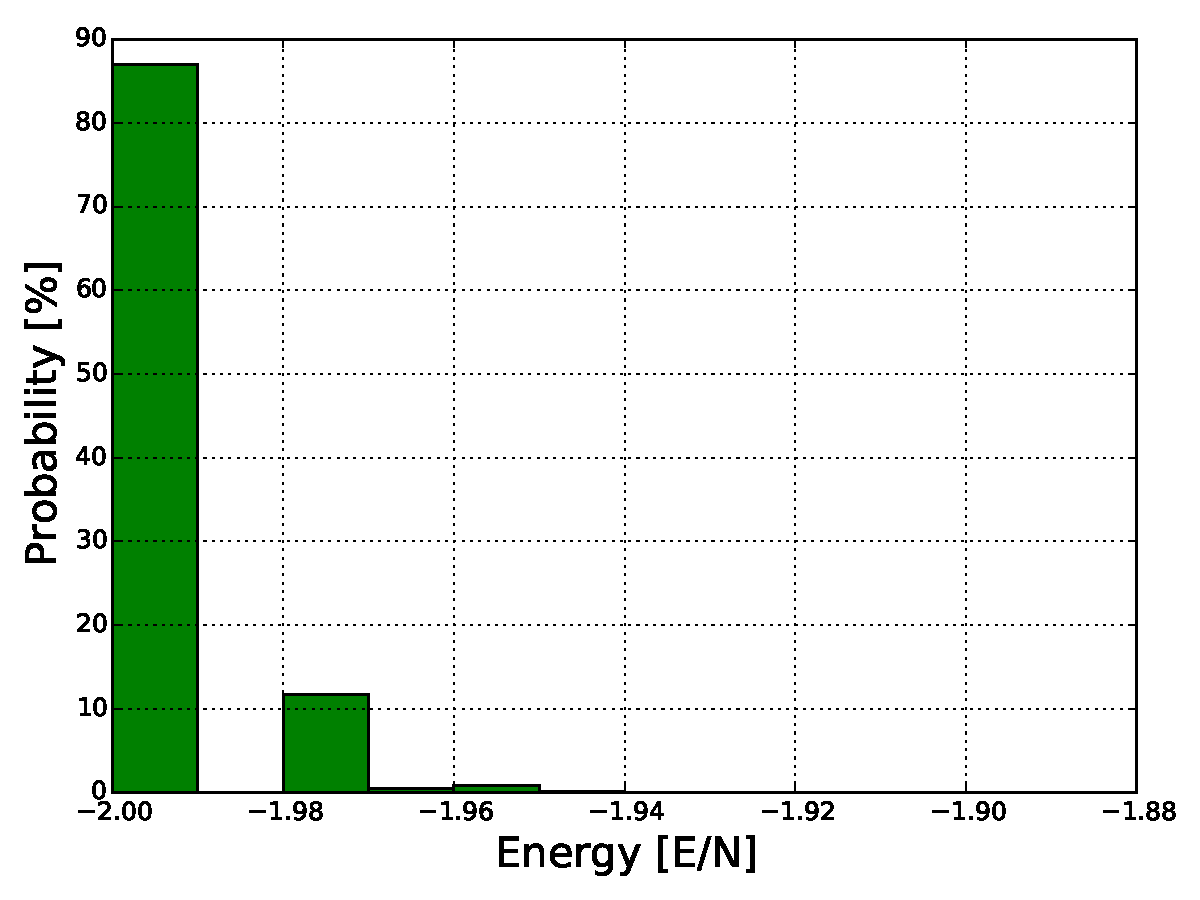
\includegraphics[width=0.5\textwidth]{MC1000000T1-distN20-hist.pdf}
		\caption{Histogram of states at T = 1 }
	\end{center}
	\end{figure}

	\begin{figure}[H]
	\begin{center}
		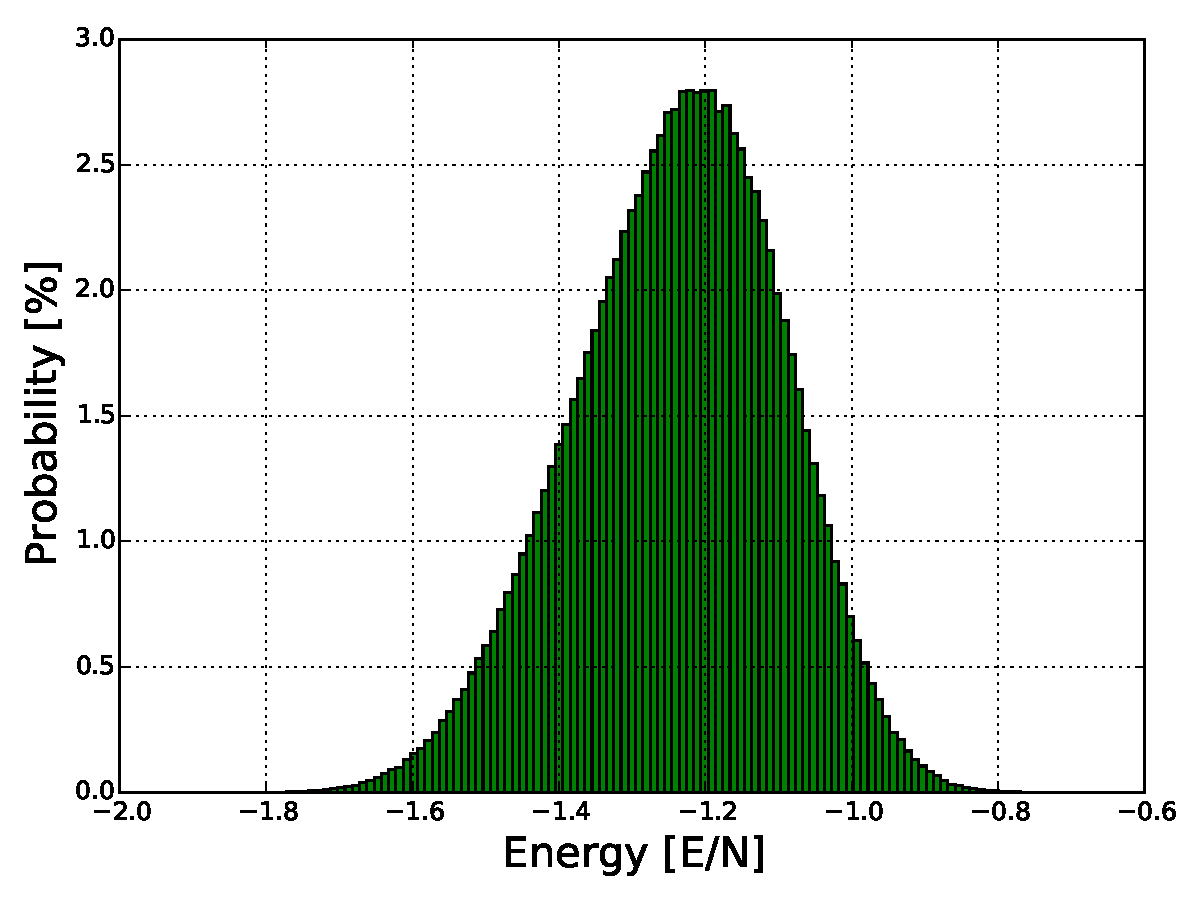
\includegraphics[width=0.5\textwidth]{MC1000000T24-distN20-hist.pdf}
		\caption{Histogram of states at T = 2.4}
	\end{center}
	\end{figure}
	We can clearly see that when the temperature is lower the system almost exclusively stays around states with a certain energy (around -2.00). While an increase in temperature leads the number of achievable states to increase drastically.

	
\newpage
\section{Conclusion}
	It is apparent that the Ising model is sufficient for explaining ferromagnetic materials. Analytical solutions of this model are tough but numerical experiments utilizing the montecarlo method are more readily available and paint an accurate depiction how ferromagnetic materials behave. The systems become more disordered at higher temperatures and the average energy increases.

\newpage
\section{Postface}
	Results and programs for this project was performed and implemented by the author and can be found at \hyperref[https://github.com/mikaelbk/fys3150-project4]{https://github.com/mikaelbk/fys3150-project4}. However, it should be noted that work on this project was done in collaboration with fellow student \hyperref[Erik Skaar]{https://github.com/erikfsk} and that certain experimental results are shared. The writing of this report was by the author only.

\begin{thebibliography}{9}
	\bibitem{schroeder}
	Daniel V. Schroeder,
	\textit{An introduction to thermal physics},
	San Francisco, Calif.: Addison Wesley Longman,
	2005
\end{thebibliography}

\end{document}